\documentclass[12pt, twocolumn]{article}

\usepackage[margin=1in]{geometry}
%\usepackage{tabularx}
\usepackage{amsmath}
\usepackage{amssymb}
%\usepackage{setspace}
\usepackage{graphicx}
\graphicspath{{./figure/}}
\usepackage{hyperref}
%\usepackage{ulem}
%\usepackage[justification=centering]{caption}
%\usepackage{parskip} % replaces parindent and parskip
%\setlength{\parindent}{0pt}
%\setlength{\parskip}{1em}
%\pagestyle{empty}
%\usepackage{slashed}
%\usepackage{simplewick}
%\usepackage{datenumber}
%\usepackage{color}
%\usepackage{multirow}
%\usepackage{feynmp} % Feynman Diagrams
%\DeclareGraphicsRule{*}{mps}{*}{} % Feynman Diagrams
%\usepackage[usenames,dvipsnames]{xcolor}
%G\usepackage[utf8]{inputenc} % for accents in the names of citation

\numberwithin{equation}{section}

\begin{document}
\sloppy % to relax the rules for inter word spacing making the word don't overflow

\title{Multi-documentation Summarization of Science Articles}
\author{Justin To, Luka Liu, Milan Dean}
\date{
    W 266: Natural language Processing
    \\UC Berkeley School of Information
    \\~
    \\\today
}
\maketitle

\begin{abstract}%\normalsize\parindent 0pt\parskip 5pt

In today's age of information overload, the ability to generate accurate and concise summaries of large amounts of text is more important than ever. This project focuses on the task of multi-document summarization (MDS), which involves automatically generating a summary that captures the main points from multiple related documents. Our approach utilizes two state-of-the-art large language models (LLMs), Centrum and LED, which are pre-trained on vast amounts of text data. We fine-tune these models on an unseen dataset of scientific papers from X-science and explore different strategies for evaluating their results. Our goal is to analyze the outputs of these fine-tuned models and evaluate their effectiveness in generating abstractive summaries, alongside evaluating a model generated by stacking the short summary output from Centrum as inputs into the LED model. By leveraging the power of these LLMs and exploring their effectiveness using the Rouge evaluation method, we aim to contribute to the growing body of research on automated text summarization and help address the ongoing challenge of information overload in scientific fields.

\end{abstract}

\section{Introduction}

Multi-document summarization is the task of summarizing multiple texts into a concise and informative summary. Moreover, it is challenging to keep the summary coherent and comprehensive, especially when the documents are long and complex. Therefore, there is a need for a system that can automatically summarize multiple related documents, providing a brief summary while avoiding hallucinations as much as possible.

In this paper, we leverage the existing multi-document summarization pre-trained models and implement an abstractive summarization system that can summarize multiple related documents into a concise and coherent summary. Realizing the multiple related documents could be very long and include long tokens, we referred to \cite{beltagy2020longformer} proposed the Reformer model for building efficient transformer-based neural networks to focus on the long former solution (LED) and \cite{puduppully2022multidocument} provided a pre-trained MDS model with Centroid-Based (Centrum) architecture.

Additionally, we extended these two pre-trained proposed multi-document summarization models on the Multi-XScience dataset~\cite{lu-etal-2020-multi-xscience}, which is a collection of scientific articles from various fields, including computer science, physics, and biology. The dataset was compiled to enable research on the summarization of scientific literature and consists of 10,000 documents from 500 different topics. Each topic contains an average of 10 documents, and each document has an average length of 1,000 words.

Lastly, we evaluated the performance of the two fine-tuned both LED and Centrum by experimenting with different training inputs, which have \texttt{num\_input\_tokens} = 512 and 4096, and compared the results of different parameters, such as \texttt{no\_repeat\_ngram\_size}. We also found that fine-tuning the models on the X-science dataset improved their performance, with the Centrum model achieving the highest ROUGE scores.

\section{Related Works}
\label{sec:relatedworks}

In recent years, there has been significant research in the field of multi-document summarization, with a particular focus on the use of transformer-based models.

The Longformer model proposed by \cite{beltagy2020longformer} addresses the issue of processing long documents by introducing a sparse attention mechanism that allows the model to scale to documents of up to 4,096 tokens in length. This approach has been shown to outperform previous models on long-document tasks such as summarization.

PRIMERA (Pyramid-based Masked Sentence Pre-training for Multi-document Summarization), proposed by Wang et al.~\cite{xiao2022primera}, is a pre-training method for transformer-based models that leverages hierarchical sentence representations to improve performance on multi-document summarization tasks. The approach involves constructing a sentence-level pyramid structure and applying a masked language modeling objective to the pyramid.

In another work, \cite{puduppully2022multidocument} propose a centroid-based pre-training method for multi-document summarization that leverages document-level clustering to capture document-level semantics. This approach has been shown to improve performance on summarization tasks, particularly for datasets with a large number of documents.

Overall, these recent developments highlight the ongoing efforts to improve the performance of transformer-based models for multi-document summarization, through approaches such as sparse attention mechanisms, hierarchical sentence representations, and document-level clustering.

\section{Methods}
\label{sec:methods}

We used the X-Science multi-source dataset \cite{lu-etal-2020-multi-xscience} to train and evaluate our LED and Centrum models for multi-document summarization because the LED model was trained based on the Multi-News dataset~\cite{fabbri-etal-2019-multi} and while the Centrum model was trained based on both the Multi-News dataset~\cite{fabbri-etal-2019-multi} and WikiSum dataset~\cite{liu2018generating}. We choose to use X-Science multi-source dataset because we like to fine-tune the LED and Centrum model to a new dataset which they were not seen in the pre-trained model.

The multi-News dataset was introduced by Fabbri et al.~\cite{fabbri-etal-2019-multi} as a multi-document summarization dataset that contains news articles from multiple sources. The dataset consists of more than 56,000 news articles and their corresponding human-generated summaries. The Wikisum dataset by Liu et al.~\cite{liu2018generating} was generated from a large-scale collection of existing Wikipedia articles.

Unlike the multi-News dataset, focusing on News or Wikisum dataset from Wikipedia, Lu et al.~introduce Multi-XScience, a large-scale dataset for extreme multi-document summarization of scientific articles~\cite{lu-etal-2020-multi-xscience}. Multi-XScience introduces a challenging multi-document summarization task: writing the related-work section of a paper based on its abstract and the articles it references, as such each summary (standard summaries) has range from 2 to 20 source documents.

Our EDA revealed that the Multi-XScience dataset contains over 40,000 datasets split among 30,369 training, 5066 validation, and 5093 test.  We also observed variations in the length and content of the articles, as demonstrated in Figure~\ref{fig:token-length}.

\begin{figure*}
    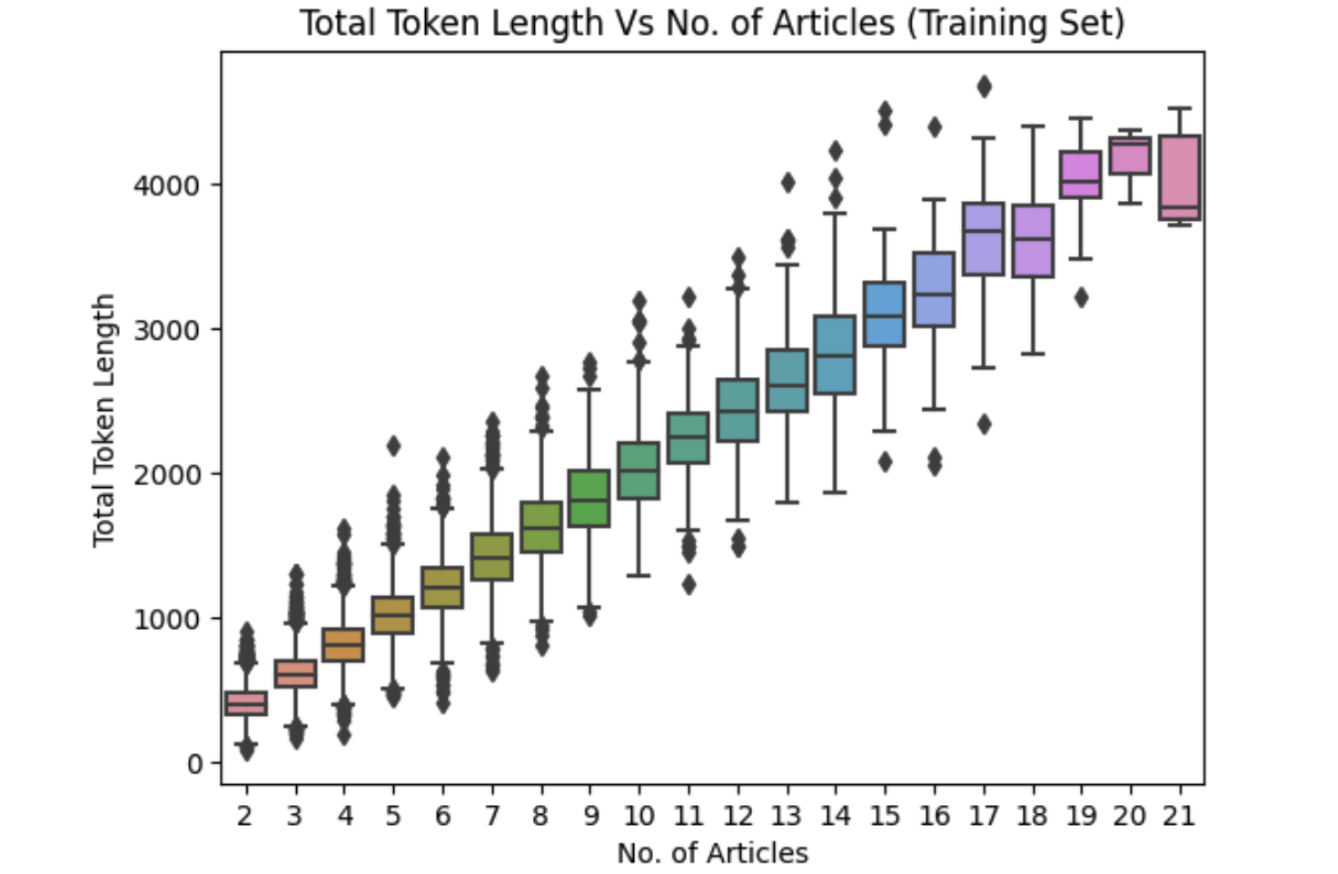
\includegraphics[width=\textwidth]{token_length.png}
    \caption{Total token length as a function of the number of articles in the training data set. The relationship between token length and the number of articles is linear.}
    \label{fig:token-length}
\end{figure*}

As mentioned above, one standard summary could be summarized from more than 20 source articles.  With concatenating all sources of articles, the total token length is about 4096. In addition, we've examined the token length of these standard summaries (label) and provided in Figure~\ref{fig:label-dist}.

\begin{figure*}
    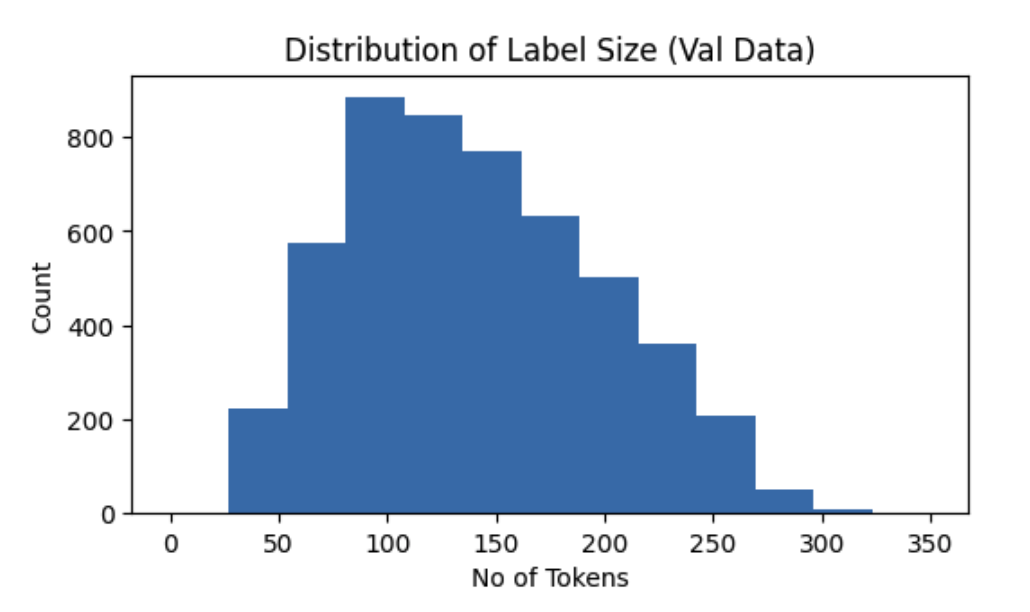
\includegraphics[width=\textwidth]{label_dist.png}
    \caption{Distribution of the number of tokens in the label of training data. The number of tokens is right-skewed and centered around 100.}
    \label{fig:label-dist}
\end{figure*}

To determine the input length, we look at the average length of the documents we want to summarize. With the consideration of the various numbers of source documents and our GPU capabilities, we decided to take input numbers of tokens = 512 as an experiment and numbers of tokens = 4096 (max tokens in the training dataset) as our final model.

For the output length, considering the desired level of detail in the summary and the distribution of standard summaries (label) tokens, we decided a summary length between 100- 250 may be sufficient.

\section{Data Preprocessing}
\label{sec:dataprocessing}

Multi-XScience includes a main abstract, which is from the main article; a standard summary of the related works with a separation of “@cite”, which is the summary of multi-source documentations, label datasets; and reference abstracts, which are the multiple abstracts from a different source of works. We processed the dataset by defining the separator of documents as ``\texttt{|||||}'', a document separator, then concatenating reference abstracts using the document separator to replace citation reference, see an example in Figure~\ref{fig:X-science-example}.

\begin{figure*}
    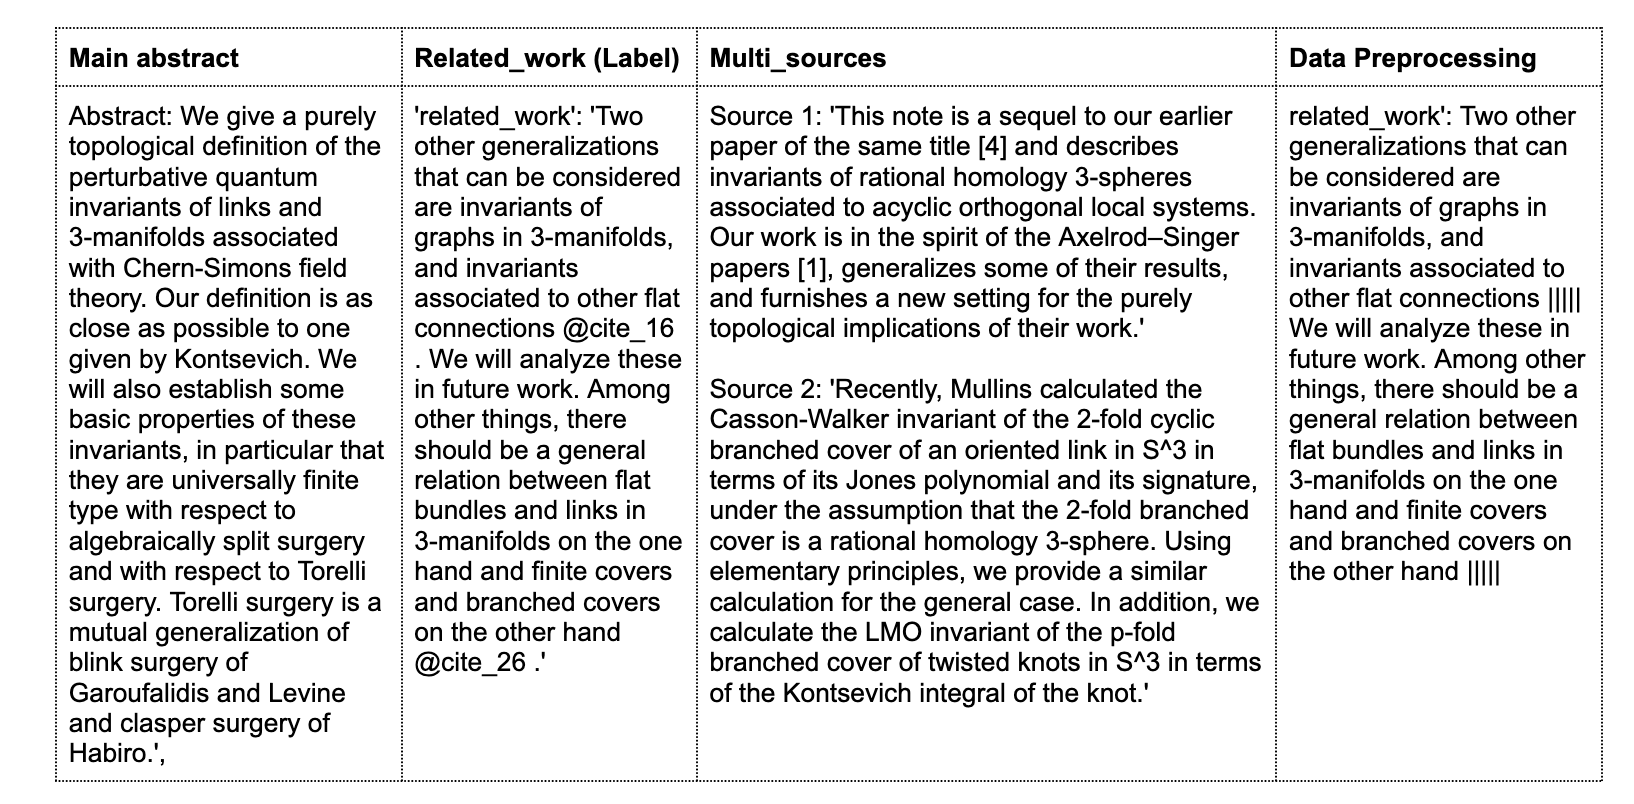
\includegraphics[width=\textwidth]{X_science_example.png}
    \caption{Data processing examples}
    \label{fig:X-science-example}
\end{figure*}


\section{Model experiments results}
\label{sec:results}

Among different metrics, we chose ROUGE-L as our primary metrics of model evaluation. Multi-document summarization is a challenging task that requires identifying the most important information from a set of related documents and producing a summary that captures the key ideas and themes from the source material. ROUGE-L is well-suited for this task because it can capture the extent to which the generated summary includes important content and maintains the same order of important words and phrases as the reference summaries. It allows us to compare the quality of the generated summaries against the reference summaries created by human experts, providing a valuable tool for evaluating and improving multi-document summarization models.

Additionally, we specifically choose the Mid ROUGE-L score, which refers to the median or average ROUGE-L score across a set of models or baselines in a given task.

We focused on pre-trained language models, which include LED and Centrum, and investigate performance differences of various models on text samples with different token lengths, and also fine-tuned based on the X-science dataset.  we conducted a series of experiments on a benchmark dataset.

\begin{enumerate}
    \item the baseline model (\ref{app:model-base-led})
    \item the baseline LED model (\ref{app:model-base-led} \& \ref{app:model-large-led})
    \item the baseline Centrum (\ref{app:model-centrum})
    \item the finetuned LED (\ref{app:model-ft-led})
    \item the finetuned Centrum (\ref{app:model-ft-centrum})
    \item the naive two-step (\ref{app:model-two-step-led} \& \ref{app:model-two-step-centrum})
\end{enumerate}
(Refer to Model Appendix for model details of each of the models)

As demonstrated in the evaluation above, our study has shown that fine-tuning the language model on summarized sources can significantly improve its performance compared to the baseline model. By leveraging LED and Centrum models to summarize related source documents and then fine-tuning the model on the summarized sources, we were able to generate more accurate and relevant summaries. These findings suggest that fine-tuning is an effective approach for improving the performance of language models in natural language processing tasks.

Additionally, we tried to experiment with a hypothesis that fine-tuned LED/Centrum model's performance could be better if they can learn based on more accurate, concise relevant sources. We leveraged the LED model to first generate a summary of each related source document to get a more concise, shorter, and summarised version. Then, generate the final summary to the fine-tuned LED/ Centrum. A schematic of this approach is shown in Figure~\ref{fig:two-steps}.

\begin{figure*}
    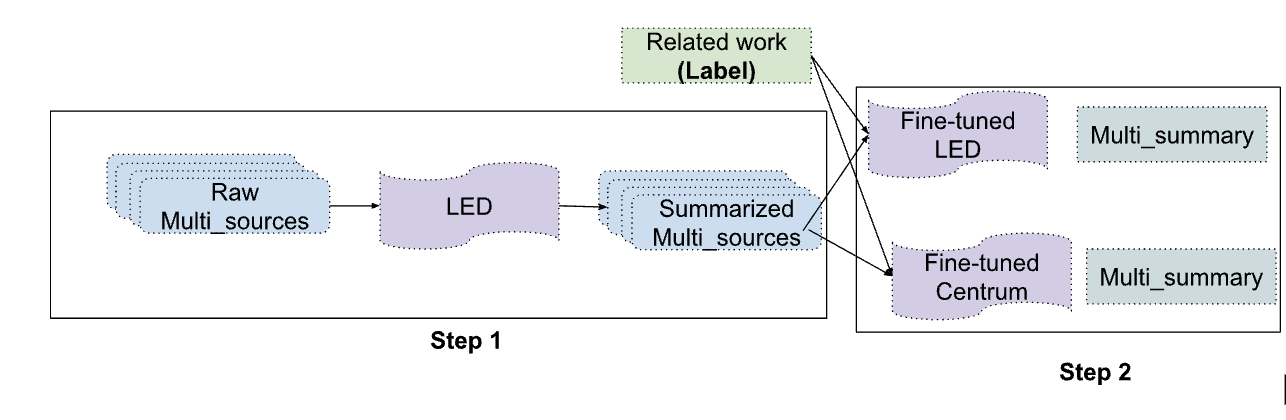
\includegraphics[width=\textwidth]{two_steps.png}
    \caption{Two-steps model design}
    \label{fig:two-steps}
\end{figure*}

In the first step, the LED model is used to generate a summary of each related source document. By summarizing each source document, the model can condense the information and reduce redundancy, making it easier to process and analyze.

In the second step, generate the summary based on the fine-tuned LED model to refine the summaries generated in the first step. In this way, we were hoping that the fine-tuned LED model can learn to generate even more accurate and relevant summaries.

However, from our evaluation and observation of this approach, the performance of the two-step model does not exceed the fine-tuned LED/Centrum model. One potential issue is that the large amount of information contained in the source documents may make it difficult for the model to generate concise and informative summaries. Ultimately, the performance is heavily dependent on the performance of step 1.

Overall, our results demonstrate the importance of utilizing advanced techniques like fine-tuning to unlock the full potential of language models in real-world applications.

\section{Quantitative Analysis}
\label{sec:quantitative}

Given that LED or Centrum is designed to process and summarize text within a certain length of the range, we want to evaluate the performance varies based on input text length. For each model, we generated summaries for samples with token lengths by 3 sets (low-length = 1st, quantile, mid-length = 1st to 3rd quantile, high-length = 3rd to 4th quantile). We then computed the ROUGEL score for each generated summary, using the related works from the dataset as the ground truth.

In our study, we found that our fine-tuned models perform better when the source articles are longer. This is because the model can leverage the additional information and context contained in longer articles to generate more accurate and informative summaries. Our findings suggest that for tasks that involve summarizing longer articles, LED may be more effective By incorporating information from multiple sources, the model can generate more accurate and informative summaries that capture the most important information from each source. Thus, this highlights the importance of considering the length and complexity of source articles.

\begin{figure*}
    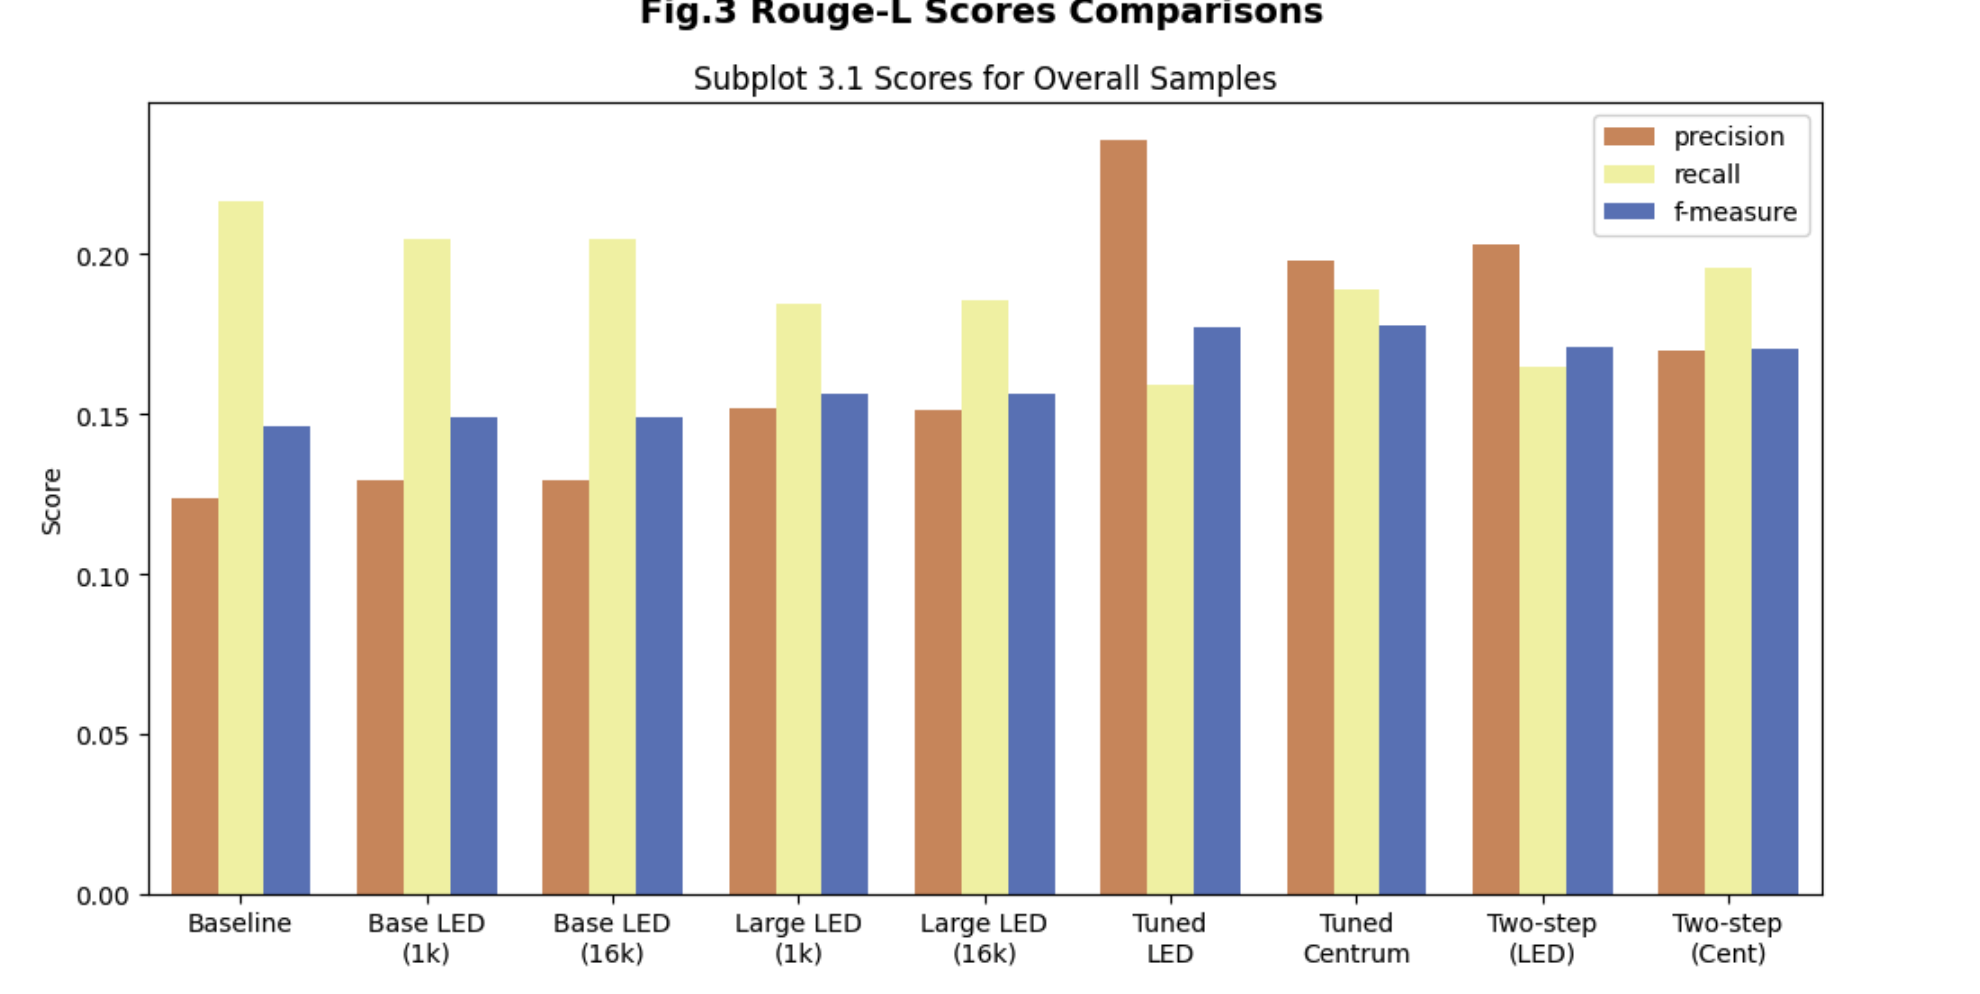
\includegraphics[width=\textwidth]{overall.png}
    \caption{ROUGE-L scores for overall samples.}
    \label{fig:overall}
\end{figure*}

\begin{figure*}
    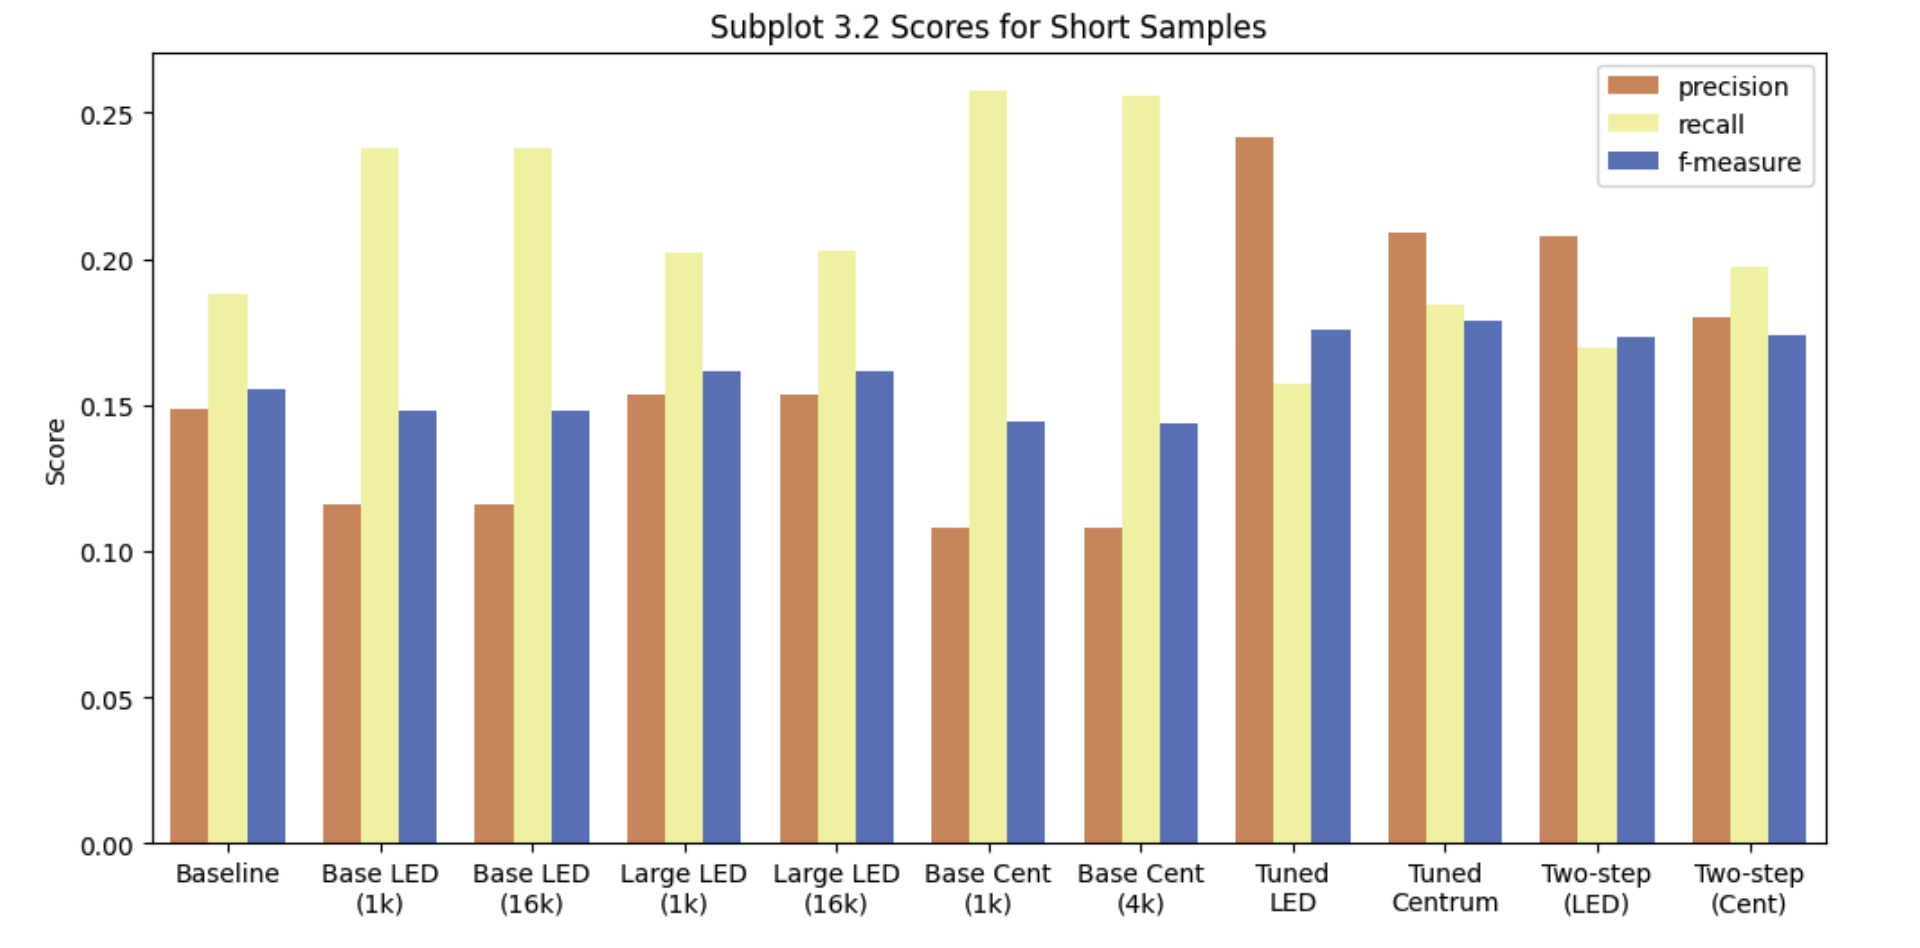
\includegraphics[width=\textwidth]{short.png}
    \caption{ROUGE-L scores for short samples.}
    \label{fig:short}
\end{figure*}

\begin{figure*}
    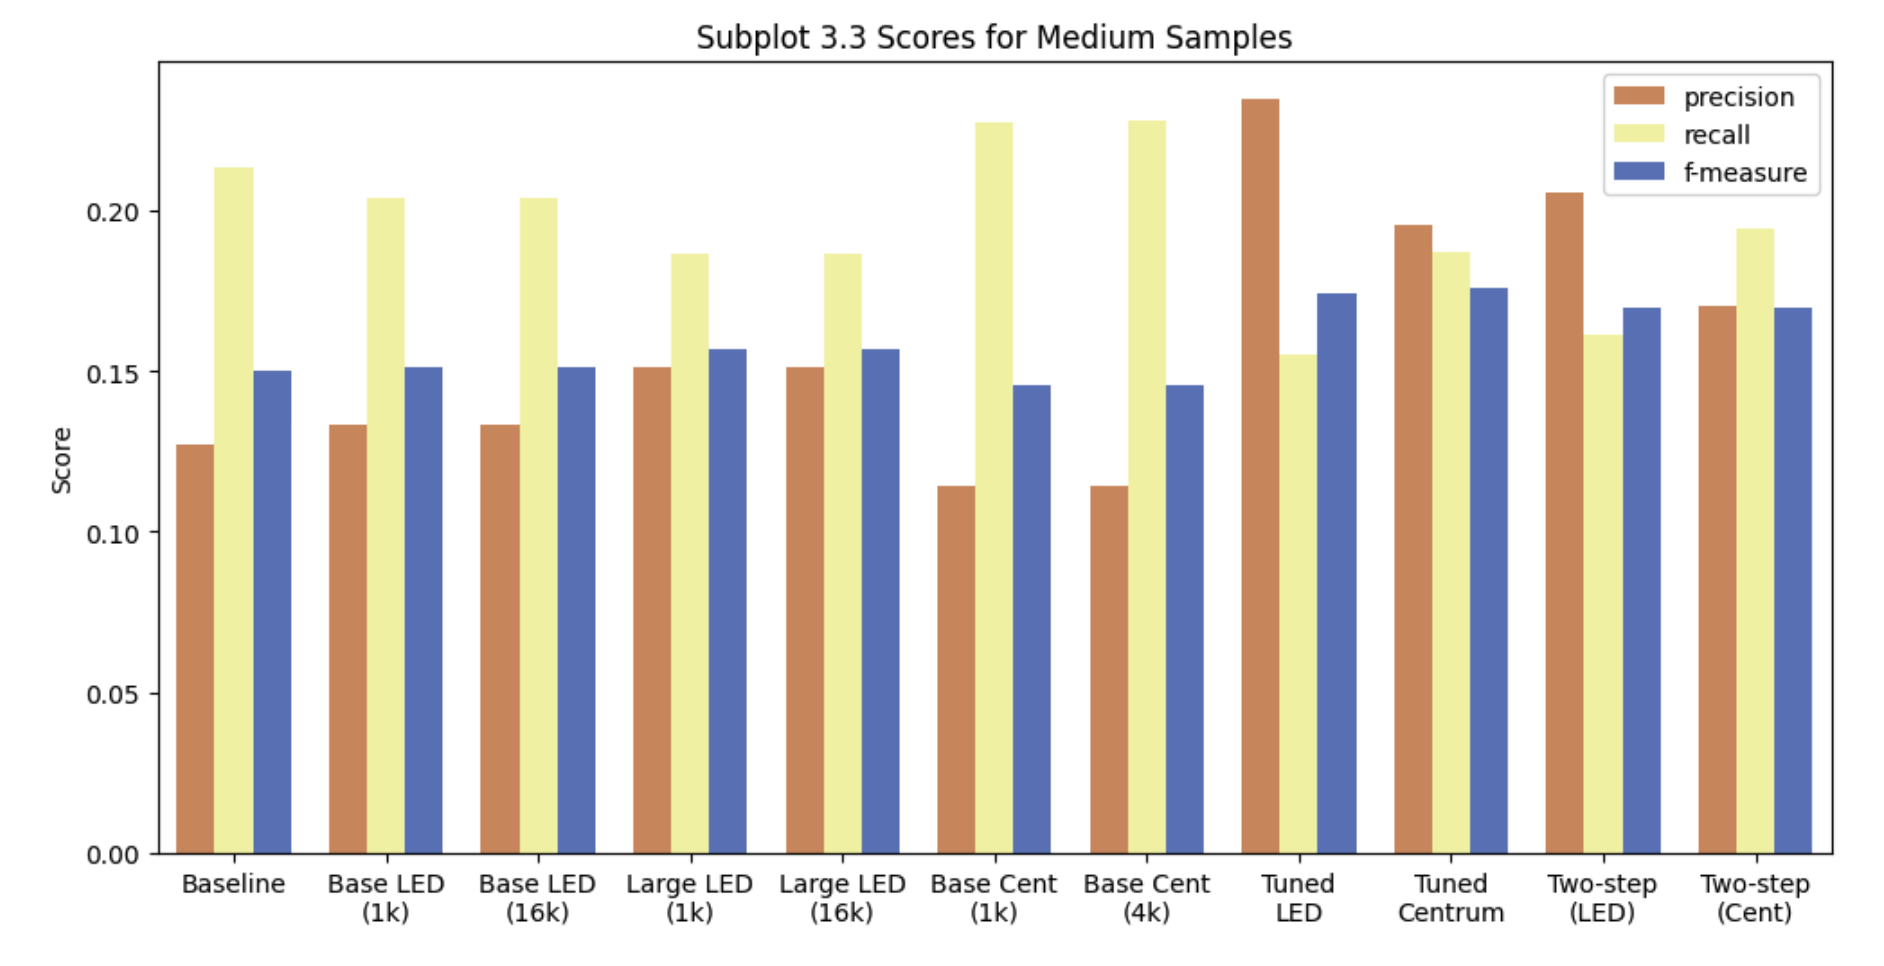
\includegraphics[width=\textwidth]{medium.png}
    \caption{ROUGE-L scores for medium samples.}
    \label{fig:medium}
\end{figure*}

\begin{figure*}
    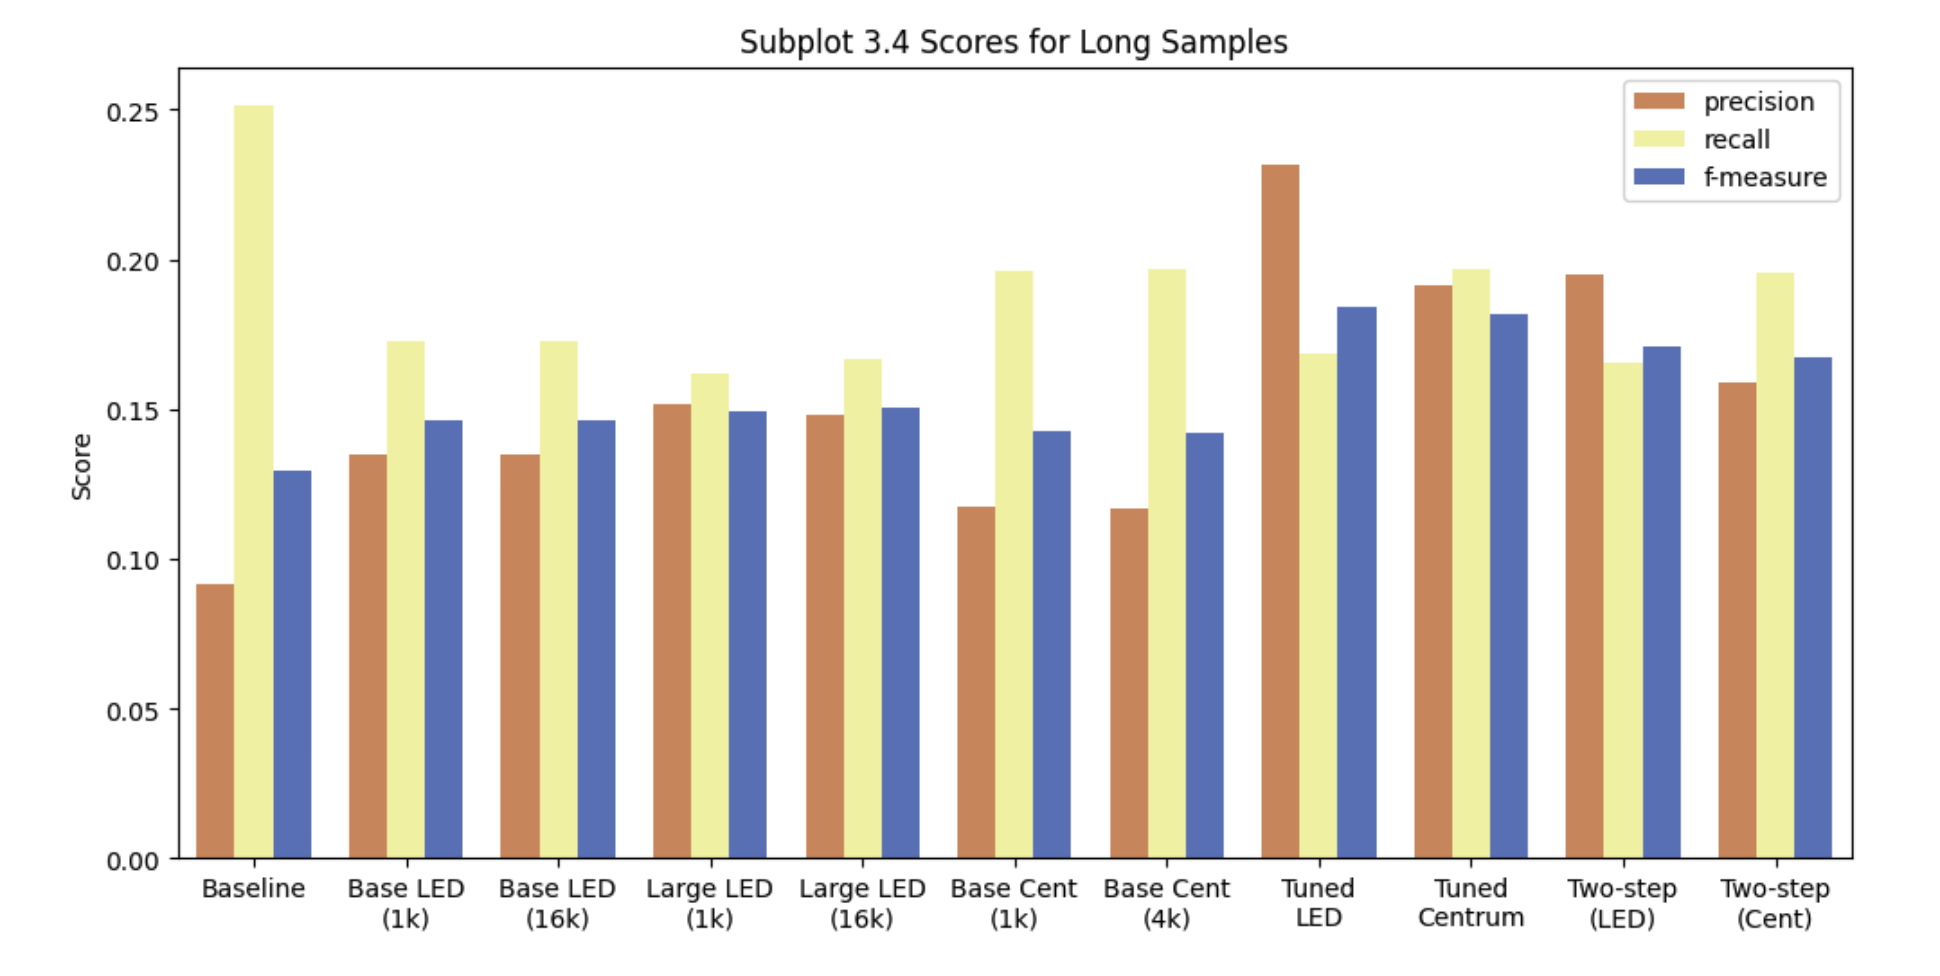
\includegraphics[width=\textwidth]{long.png}
    \caption{ROUGE-L scores for long samples.}
    \label{fig:long}
\end{figure*}

\begin{figure*}
    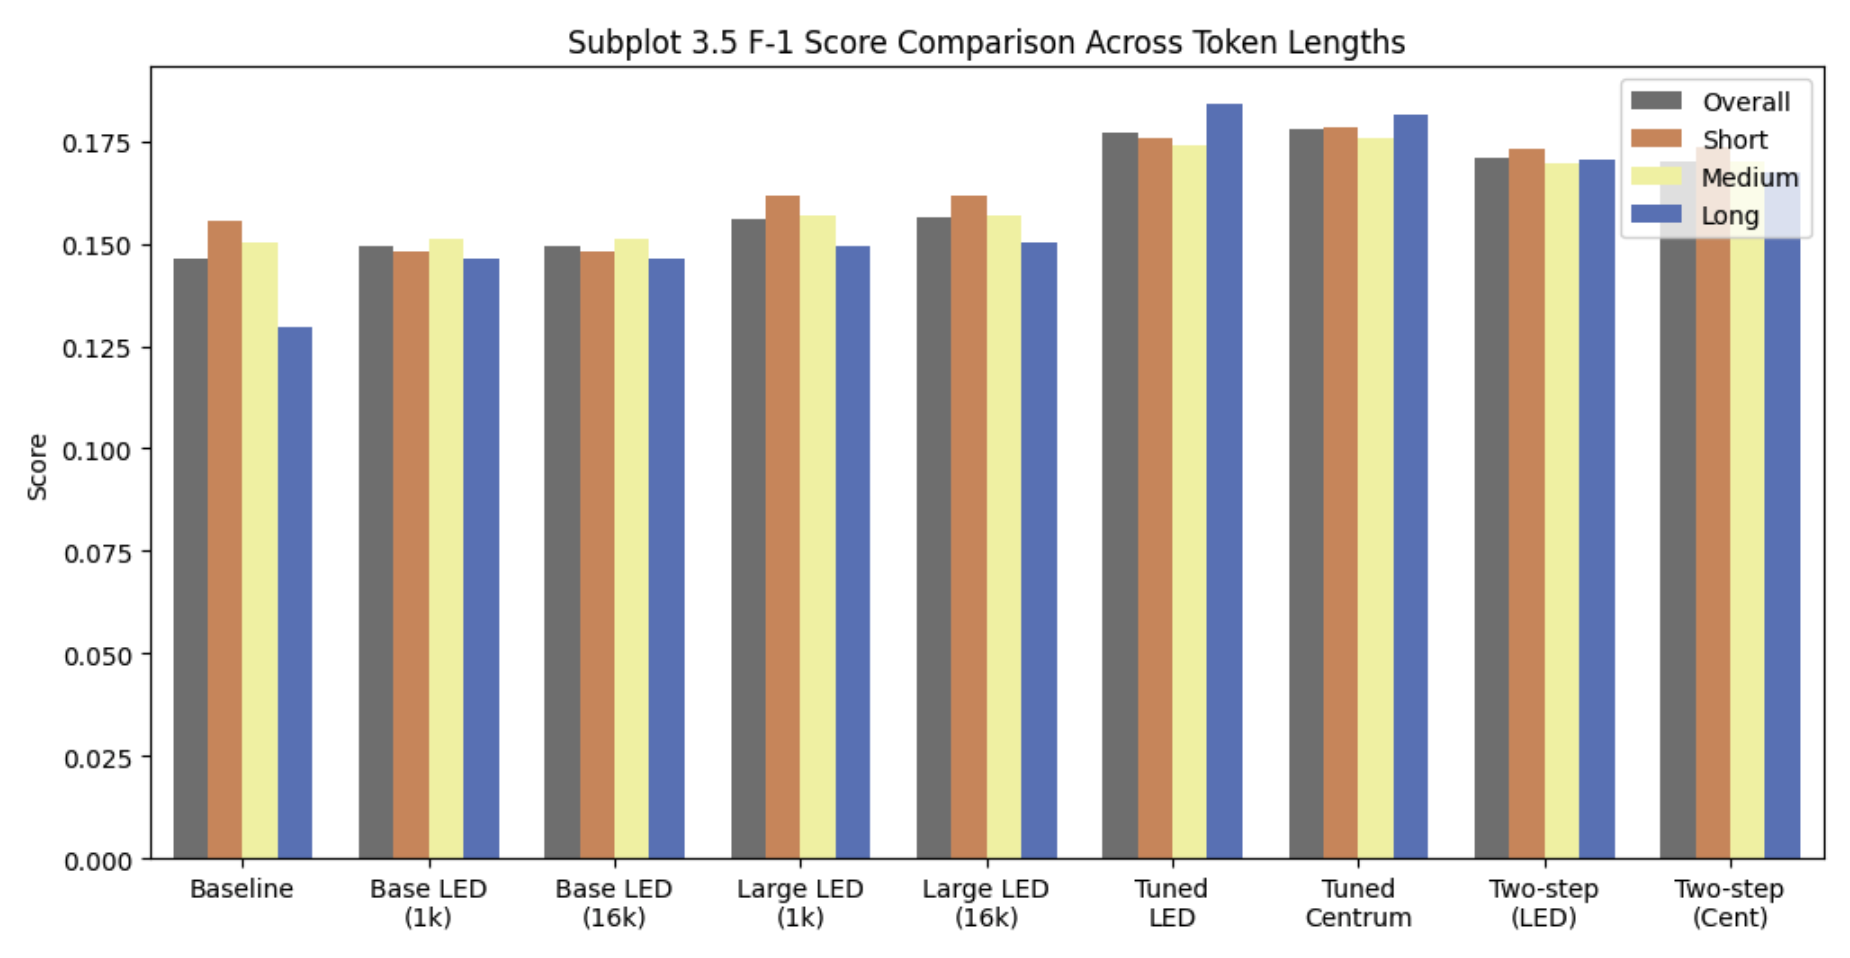
\includegraphics[width=\textwidth]{various_lengths.png}
    \caption{ROUGE-L scores comparison across token lengths.}
    \label{fig:various-length}
\end{figure*}

\section{Qualitative Analysis}
\label{sec:qualitative}

We also investigated how the model performed when summarizing short, medium, and long documents. The study aimed to evaluate the quality of the generated summaries and identify any trends or patterns in the model's performance based on the length of the source documents. A total of 25 randomly drawn samples (from the 5093 samples in the X-Science test dataset) are analyzed.  These 25 samples include:

\begin{itemize}
    \item 10 short samples, i.e. with total token lengths below the lower quartile
    \item 10 medium samples, i.e. with total token lengths between the lower and upper quartiles
    \item 5 long samples, i.e. with token lengths above the upper quartile
\end{itemize}

Our analysis of the review (refer to the Analysis Appendix for more detail review) results showed that the fine-tuned LED and Centrum learned the structure for multi-documents summary for X-science dataset, with particularly good results for longer documents (ref. Sample no 4263, 76, 485, 1864) while the shorter samples seems extract the main abstract and add another journal abstract without a strong indication of multi-document summarization (ref. Sample no 556, 483).

Additionally, we observed that LED and Centrum seems to have difficulties in digesting math topics, where the use of common language for unusual meanings might have confused the models (refer to no 4820, 638, 4717).  The two-step model somehow helps for these samples, but the downside is that the two-step model hallucinates quite a bit. In general, LED and Centrum never really hallucinates. To future improve this issue, we would suggest the further research in this area should consider:

\begin{itemize}
    \item Add domain-specific knowledge: This can include adding specialized math dictionaries or knowledge bases to your training data.
    \item Use special tokens for math symbols: This can help the model recognize and differentiate between mathematical expressions and regular language. For example, use a special token such as "[math]" to indicate the start of a math expression and "[/math]" to indicate the end.
    \item Use more training data: Consider adding more math-specific data to the training set to help the model learn to recognize and understand math concepts.
    \item Fine-tune your model: fine-tuning it on a smaller dataset of math-specific documents. This can help the model learn to recognize and summarize math-related information more effectively.
\end{itemize}

Overall, our study highlights the importance of considering the length of source documents, and the training datasets topics when evaluating the performance of multi-document summarization models.

Future research in this area should focus on developing models that can effectively summarize long documents; and provide the model with more specialized knowledge to help the model recognize and differentiate between regular language and math expressions, improving its ability to summarize math-related documents effectively.

\section{Conclusion}
\label{sec:conclusion}

In conclusion, our experiments demonstrate the importance of considering the token length of input texts when selecting a text summarization model. Our results suggest that the finetuned LED and Centrum models may be more effective for summarizing longer texts, while the naive two-step model may be sufficient for shorter texts and help a bit with specialized math topics. Future work could explore more sophisticated summarization approaches for longer texts, to further improve the performance of automated text summarization systems.

\appendix

\section{Model}
\label{app:model}

\subsection{Baseline Model}
\label{app:model-baseline}

Copying the first 3 sentences from each reference abstract was used as our baseline. It is a simple and easy-to-implement approach that provides a starting point for summarizing multiple documents. It assumes that the first few sentences of a document contain important information that should be included in the summary.

This approach can serve as a useful baseline for several reasons:

\begin{itemize}
    \item It is easy to implement and does not require a lot of computational resources. This makes it a good starting point for developing more advanced summarization models.
    \item It is straightforward to understand and explain. This makes it a good choice for initial experiments and evaluations.
    \item It can provide a quick estimate of the performance of a summarization system. By comparing the summaries generated by this approach to human-written summaries or other machine-generated summaries, it is possible to get a rough idea of how well the system is performing.
\end{itemize}

\subsection{Baseline Base LED (1K and 16K) Model}
\label{app:model-base-led}

The base LED model has (“allenai/led-base-16384”), with max input token length of 16384 \& $\sim$200M parameters and consists of 12 transformer encoder layers and 2 transformer decoder layers. This model is designed to be computationally efficient and suitable for low-resource environments. The baseline LED was generated based on a pre-trained LED model by \cite{beltagy2020longformer} on X-science test datasets with input tokens varying from 1k and 6k.

\subsection{Baseline Large LED (1K and 16K) Model}
\label{app:model-large-led}

The "large" in the model name indicates that it has more parameters and is larger than the "base" LED model. The model has (“allenai/led-large-16384-arxiv”), with max input token length of 16384 \& $\sim$512M parameters and consists of 24 transformer encoder layers and 4 transformer decoder layers. This model has been pre-trained for general summarization task. The baseline LED was generated based on a pre-trained large LED and evaluated on X-science test datasets.

\subsection{Baseline Centrum Model}
\label{app:model-centrum}

The "ratishsp/Centrum" model with max input token length of 4096 \& $\sim$192M parameters and consists of 12 transformer encoder layers and 12 transformer decoder layers. It is smaller than some of the larger transformer models, such as T5 and GPT-3, but larger than some of the smaller transformer models, such as BART base. The publicly available Centrum checkpoint was built upon the LED model architecture using the 4096 token version.This means Centrum is not able to take in 16384 tokens.

\subsection{Fine-tuned LED Model}
\label{app:model-ft-led}

Fine-tuning the "LED-large-16384-arxiv" model to the X-science train (size 30369) and validation (size 5066) datasets specifically for the related work summarization. We used 4096 max number of tokens in tracking and validation sets, and 256 max output tokens with a batch size of 2 (due to limited GPU resources). The model is then used as a cross-entropy loss function for 2 epochs, and evaluated on test datasets(size 5093) with ROUGE metrics.

\subsection{Fine-tuned Centrum Model}
\label{app:model-ft-centrum}

Fine-tuning the"ratishsp/Centrum" model to the X-science train and validation datasets specifically for the related works summarization. We used 4096 max number of tokens in tracking and validation sets, and 256 max output tokens with a batch size of 16 (due to limited GPU resources). The model is then used as a cross-entropy loss function for 2 epochs, and evaluated on test datasets with ROUGH metrics.

\subsection{Two-step LED Model}
\label{app:model-two-step-led}

In the first step, the LED model is used to generate a summary of each related source document. By summarizing each source document, the model can condense the information and reduce redundancy, making it easier to process and analyze. For the first step, none of the individual source articles in the X-science dataset contain more than 4096 tokens, so there is no issue of the first step model (i.e.~the finetuned LED) receiving truncated inputs.

In the second step, generate the summary based on the fine-tuned LED model to refine the summaries generated in the first step. In this way, we were hoping that the fine-tuned LED model can learn to generate even more accurate and relevant summaries.

\subsection{Two-step Centrum Model}
\label{app:model-two-step-centrum}

The same first step as the two-step LED Model above. In the second step, generate the summary based on the fine-tuned Centrum model to refine the summaries generated in the first step. In this way, we were hoping that the fine-tuned Centrum model can learn to generate even more accurate and relevant summaries.

\section{Analysis}
\label{app:analysis}

Refer to the \href{https://drive.google.com/file/d/1sPLj4a-rafh1EjOR7l_QMveexfoaxq3y/view?usp=share_link}{link}.

{
    \footnotesize
    %{\scriptsize
    \bibliography{bibliography}
    \bibliographystyle{plain}
}

\end{document}
